\section{Modélisation}
\label{sec:filtres/mode}

Dans cette section, nous allons commencer par analyser les filtres
par une bonne intuition,
ensuite nous poserons nos hypothèses de modélisation,
puis nous trouverons les fonctions de transfert et en extrairons
les expressions des gains et amplitudes,
et enfin nous interpréterons les résultats.

\subsection{Intuition}
\label{subsec:filtres/mode/intuition}

Le filtre passe-haut comme le filtre passe-bas
consistent en une capacité et une résistance en série,
avec une tension forcée aux bouts.

Prenons une analogie hydraulique:
les tensions deviennent des différences de pressions
et les courants deviennent des débits.
On peut voir la capacité comme une large membrane élastique
tendue par les déplacements d'eau;
et la résistance comme un fin tuyau
qui requiert une plus grande pression pour un même débit.
La source est une pompe qui crée une différence de pression.

Pour de basses fréquences, la pression oscille doucement.
La membrane de la capacité à donc bien le temps de s'équilibrer avec elle,
tandis que la pression à travers le fin tuyau sera petite.

Pour de hautes fréquences, au contraire,
la pression oscille très rapidement.
La membrane n'a donc pas le temps d'être tendue par le débit,
et toute la différence de pression
se trouvera aux extrémités du fin tuyau.

En conclusion, on s'attend à ce que le filtre passe-haut,
qui prend la tension aux bornes de la résistance (fin tuyau),
atténue les basses fréquences et conserve les hautes fréquences;
et à ce que le filtre passe-bas,
qui prend la tension aux bornes de la capacité (membrane),
conserve les basses fréquences et atténue les hautes fréquences.

\subsection{Hypothèses}

Pour modéliser la réponse des filtres à différents signaux nous allons utiliser
la méthode des phaseurs, comme décrite dans l'annexe~\ref{chap:phaseurs}.
Nous supposerons donc ici que le signal est une sinusoïde pure, les autres cas
pouvant s'y ramener en prenant la transformée de Fourier.

Nous supposons également que tous les composants et les liaisons entre eux
sont idéaux.
En particulier, nous considérons que les courants d'entrée de l'ampli-op
et l'ampli audio sont négligeables.

\subsection{Résolution}

Définissons comme sur la figure~\ref{fig:filtres-v1v2v3}
$V_1$, $V_2$, et $V_3$ les phaseurs des tensions
à l'entrée, après le filtre passe-haut, et après le filtre passe-bas.
Pour une explication des phaseurs, voir l'annexe~\ref{chap:phaseurs},
et plus particulièrement la section~\ref{sec:phaseurs/impedance}.

Tout le courant passant à travers le condensateur $C_2$ passe
aussi à travers la résistance $R_2$.
Par conséquent, on peut appliquer la loi de division des tensions,
avec les impédances $\frac{1}{j\omega C_2}$ et $R_2$:
\begin{equation}
    V_2\,/\,V_1
    = \frac{R_2}{\frac{1}{j\omega C_2} + R_2}
    = \frac{j\omega R_2C_2}{1+j\omega R_2C_2}
\end{equation}
Ce rapport est appelé \emph{fonction de transfert}, et nous le notons
$H\ind{ph}(j\omega)$.

Pour le filtre passe-bas, de la même manière, tout le courant
passant à travers la résistance $R_3$ passe aussi à travers le
condensateur $C_3$, donc on peut appliquer
la loi de division des tensions avec les impédances
$R_3$ et $\frac{1}{j\omega C_3}$:
\begin{equation}
    V_3\,/\,V_2
    = \frac{\frac{1}{j\omega C_3}}{\frac{1}{j\omega C_3} + R_3}
    = \frac{1}{1+j\omega R_3C_3}
\end{equation}
que nous notons $H\ind{pb}(j\omega)$.

Étant donné que la tension $V_2$ est répétée de la sortie du filtre passe-haut
à l'entrée du filtre passe-bas, la fonction de transfert totale du système est:
\begin{align}
    H\ind{tot}(j\omega) &= H\ind{ph}(j\omega)\,H\ind{pb}(j\omega) =
    \frac{j\omega R_2C_2}{1 + j\omega R_2C_2}\,\cdot\,
    \frac{1}{1 + j\omega R_3C_3}\\
    &= \frac{j\omega R_2C_2}{1 + j\omega\,(R_2C_2+R_3C_3) +
        (j\omega)^2\,(R_2C_2R_3C_3)}
\end{align}

\subsection{Gain et déphasage}

Nous allons maintenant déterminer
le \emph{gain} (rapport d'amplitude) et le  \emph{déphasage} (décalage)
entre l'entrée et la sortie de chacun des filtres.
Ils correspondent respectivement au module et à l'argument de la fonction de
transfert.

C'est-à-dire, pour le filtre passe-haut:
\begin{align}
    G\ind{ph}(\omega) &= |H\ind{ph}(j\omega)|
    = \frac{|j\omega R_2C_2|}{|1 + j\omega R_2C_2|}
    = \frac{\omega R_2C_2}{\sqrt{1+(\omega R_2C_2)^2}}\\
    \phi\ind{ph}(\omega) &= \arg\big(H\ind{ph}(j\omega)\big)
    %= \arctan(j\omega R_2C_2) - \arctan(1+j\omega R_2C_2)
    = \arctan\left(\frac{1}{\omega R_2C_2}\right)
\end{align}
et pour le filtre passe-bas:
\begin{align}
    G\ind{pb}(\omega) &= |H\ind{pb}(j\omega)|
    = \frac{|1|}{|1 + j\omega R_3C_3|}
    = \frac{1}{\sqrt{1+(\omega R_3C_3)^2}}\\
    \phi\ind{pb}(\omega) &= \arg\big(H\ind{pb}(j\omega)\big)
    = \arctan(-\omega R_3C_3)
\end{align}

\begin{figure}[h!]
    \centering
    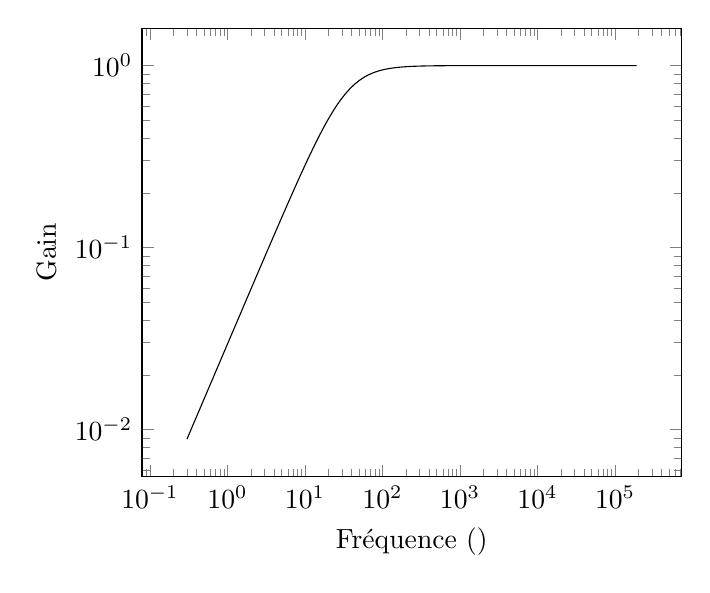
\begin{tikzpicture}
        \begin{loglogaxis}[
                xlabel={Fréquence (\hertz)},
                ylabel={Gain},
            ]
            \addplot[domain=0.3:1.9e5,samples=100]
            {1 / sqrt(1+1/(2*pi*10e3*470e-9*x)^2)};
        \end{loglogaxis}
    \end{tikzpicture}
    \qquad
    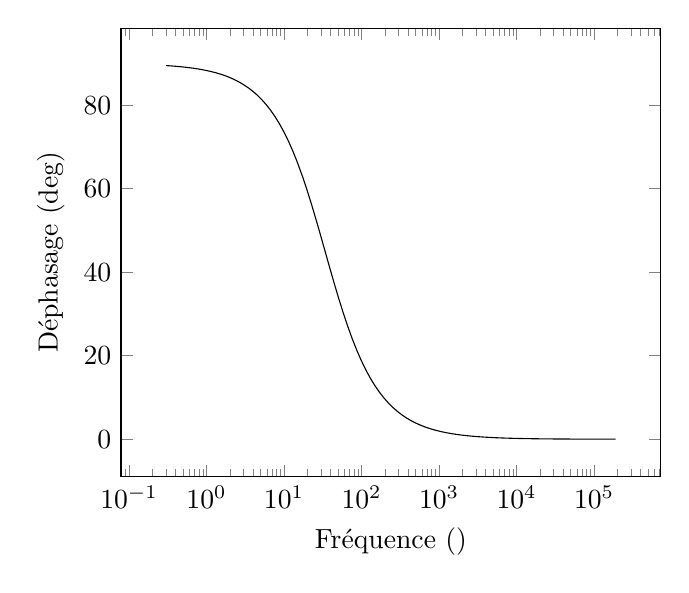
\begin{tikzpicture}
        \begin{semilogxaxis}[
                xlabel={Fréquence (\hertz)},
                ylabel={Déphasage (deg)},
            ]
            \addplot[domain=0.3:1.9e5,samples=100]
            {atan(1/(2*pi*10e3*470e-9*x)};
        \end{semilogxaxis}
    \end{tikzpicture}
    \caption{Courbes caractéristiques du filtre passe-haut}
    \label{fig:graphes-ph}
\end{figure}

\begin{figure}[h!]
    \centering
    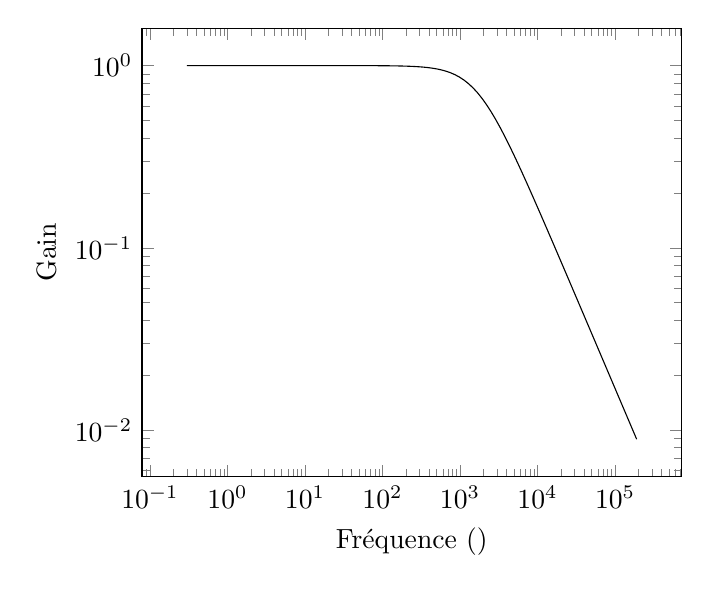
\begin{tikzpicture}
        \begin{loglogaxis}[
                xlabel={Fréquence (\hertz)},
                ylabel={Gain},
            ]
            \addplot[domain=0.3:1.9e5,samples=100]
            {1 / sqrt(1+(2*pi*200*470e-9*x)^2)};
        \end{loglogaxis}
    \end{tikzpicture}
    \qquad
    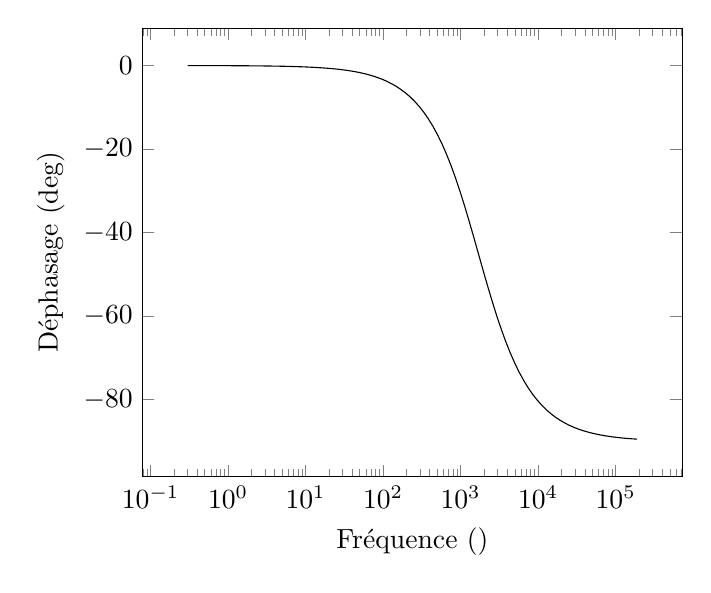
\begin{tikzpicture}
        \begin{semilogxaxis}[
                xlabel={Fréquence (\hertz)},
                ylabel={Déphasage (deg)},
            ]
            \addplot[domain=0.3:1.9e5,samples=100]
            {atan(-2*pi*200*470e-9*x)};
        \end{semilogxaxis}
    \end{tikzpicture}
    \caption{Courbes caractéristiques du filtre passe-bas}
    \label{fig:graphes-pb}
\end{figure}

Ces résultats sont illustrés par des graphes dans
les figures~\ref{fig:graphes-ph} et~\ref{fig:graphes-pb},
avec en abscisse la pulsation
et en ordonnée le gain et le déphasage.
Les tendances découvertes sont en pointillés.
Ici, le potentiomètre 2 est réglé à $20\,\%$ et le 3 à $100\,\%$,
donc $R_2 = 200\,\ohm$ et $R_3 = 2\,\kilo\ohm$.

Nous utilisons une échelle logarithmique pour les fréquences
ou pulsations, ainsi que pour les gains.
Les raisons de ce choix sont expliquées dans
la section~\ref{subsec:approx-lin/pres/loglog}.

Enfin, pour la combinaison des deux filtres,
les fonctions de transfert sont multipliées,
donc les gains sont multipliés et les déphasages sont additionnés.%
\footnote{
    Cela découle des propriétés du module et de l'argument.
    En effet, pour des complexes $x$ et $y$,
    on a $|xy| = |x||y|$ et $\arg(xy) = \arg x + \arg y$.
}
Le résultat est illustré dans la figure~\ref{fig:graphes-bande}.

\begin{figure}[h!]
    \centering
    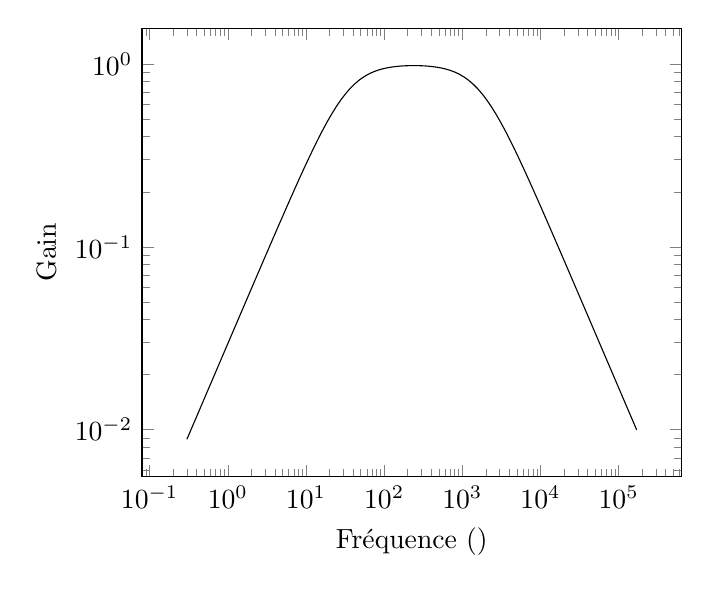
\begin{tikzpicture}
        \begin{loglogaxis}[
                xlabel={Fréquence (\hertz)},
                ylabel={Gain},
            ]
            \addplot[domain=0.3:1.7e5,samples=100]
            {1 / sqrt(1+1/(2*pi*10e3*470e-9*x)^2)
                / sqrt(1+(2*pi*200*470e-9*x)^2)};
        \end{loglogaxis}
    \end{tikzpicture}
    \qquad
    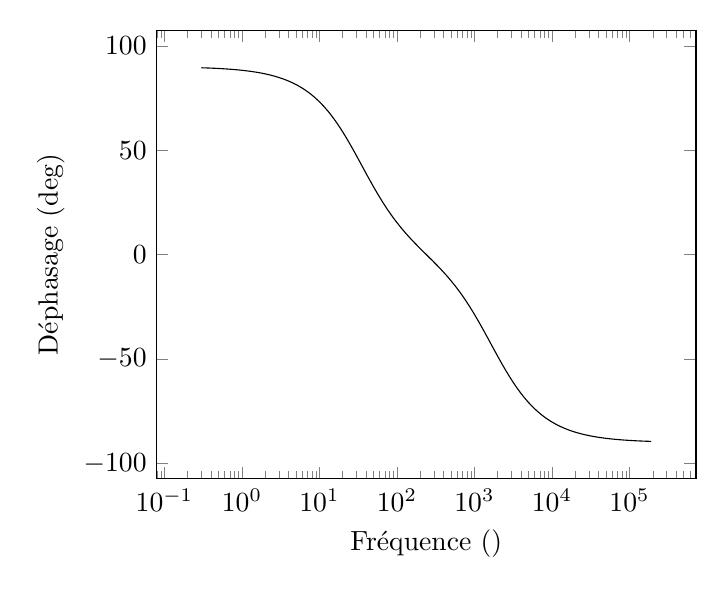
\begin{tikzpicture}
        \begin{semilogxaxis}[
                xlabel={Fréquence (\hertz)},
                ylabel={Déphasage (deg)},
            ]
            \addplot[domain=0.3:1.9e5,samples=100]
            {atan(1/(2*pi*10e3*470e-9*x))+atan(-2*pi*200*470e-9*x)};
        \end{semilogxaxis}
    \end{tikzpicture}
    \caption{Courbes caractéristiques de la combinaison des deux filtres}
    \label{fig:graphes-bande}
\end{figure}

Nous noterons les pulsations de coupure
$\omega\ind{bas} = 1/R_2C_2$ et $\omega\ind{haut}=1/R_3C_3$,%
\footnote{Nous omettrons les parenthèses lorsque cela améliore la lisibilité.}
appelées \emph{pulsations de coupure}.
Elles indiquent le passage d'un comportement à l'autre.
Nous expliquerons l'origine de ces valeurs en détail dans
l'annexe~\ref{chap:filtres-gen}.

\subsection{Interprétation}

\textbf{\textsc{À réécrire et compléter}}

Nous pouvons voir dans la figure~\ref{fig:graphes-bande}
que notre combinaison de filtres a bien le résultat attendu.
En effet, on voit que les signaux dont les pulsations sont dans l'intervalle
$[\omega\ind{bas},\omega\ind{haut}]$
\footnote{Ou dont les fréquences sont dans l'intervalle
    $[f\ind{bas},f\ind{haut}]$ avec
    $f\ind{bas} = \omega\ind{bas}/2\pi$ et
    $f\ind{haut} = \omega\ind{haut}/2\pi$.}
sont conservées.

La première remarque à faire est que les filtres ne sont pas des filtres idéaux
en ce sens que la coupure de signal n'est pas brutale:
dans le filtre passe-haut comme dans le filtre passe-bas,
l'amplitude décroit linéairement en échelle log-log.
Cela dit, ce n'est pas forcément une mauvaise chose.
En effet, cela permet d'atténuer certaines fréquences sans pour autant
les supprimer complètement.

